\begin{frame}[c]
  \myframetitle{Aufgabe 2}{Suche mittels HITS}
\begin{itemize}
  \item Berechnet die Wahrscheinlichkeit das eine Seite ein Hub oder eine Authority ist
  \item Muss bei jeder Suchanfrage neu berechnet werden
  \item In der Übung wurde die Iterative Methode verwendet
  \item Der Algorithmus terminiert meistens nach 11 Iterationen
\end{itemize}
\end{frame}

\begin{frame}[c]
    \myframetitle{HITS}{Authority ist hoch bei vielen eingehenden Links}
    %\usepackage{graphics} is needed for \includegraphics
\begin{figure}[htp]
\begin{center}
  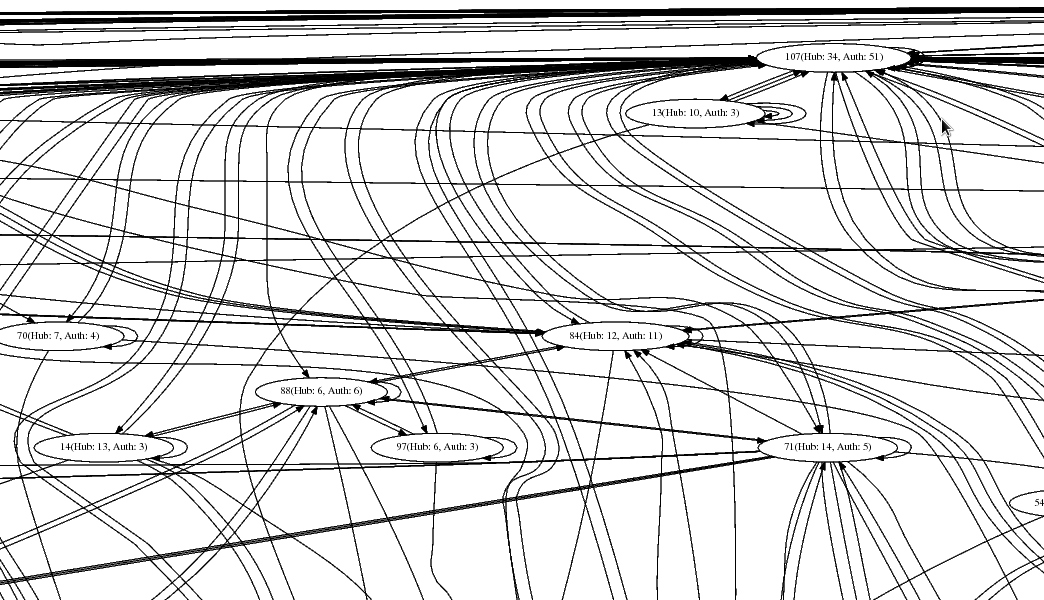
\includegraphics[height=1\textheight]{graphics/hitsGraph.png}
%  \caption[labelInTOC]{}
%  \label{fig:hihg_inoutdegree}
\end{center}
\end{figure}

\end{frame}